\documentclass[12pt,letterpaper]{hmcpset}
\usepackage[margin=1in]{geometry}
\usepackage{graphicx}
\usepackage{siunitx}

% info for header block in upper right hand corner
\name{ }
\class{Math 60}
\assignment{HW 10}
\duedate{Tuesday, May 31, 2016}

\newcommand{\f}[2]{\frac{#1}{#2}}
\newcommand{\pn}[1]{\left(#1\right)}
\newcommand{\abs}[1]{\left|#1\right|}
\newcommand{\bk}[1]{\left[#1\right]}
\renewcommand{\bf}[1]{\mathbf{#1}}
\renewcommand{\labelenumi}{{(\alph{enumi})}}

\begin{document}

\problemlist{6.1.\{2, 9, 21, 31, 34, 40\}}

\begin{problem}[Colley 6.1.2]
    In Exercises 2-7, calculate $\int_{\bf{x}}f~ds$, where $f$ and
    $\bf{x}$ are as indicated.
    \[
        f(x,y,z)=xyz,\quad\bf{x}(t)=(t,2t,3t),\quad0\leq t\leq2
    \]
\end{problem}
\begin{solution}
    \vfill
\end{solution}
\newpage

\begin{problem}[Colley 6.1.9]
    In Exercises 8-16, find $\int_{\bf{x}}\bf{F}\cdot d\bf{s}$, where the
    vector field $\bf{F}$ and the path $\bf{x}$ are given.
    \[
        \bf{F}=(y+2)~\bf{i}+x~\bf{j},\quad\bf{x}(t)=(\sin t,-\cos t),
        \quad0\leq t\leq\pi/2
    \]
\end{problem}
\begin{solution}
    \vfill
\end{solution}
\newpage

\begin{problem}[Colley 6.1.21]
    Let $\bf{F}=(x^2+y)\bf{i}+(y-x)\bf{j}$ and consider the two paths
    \begin{align*}
        \bf{x}(t)&=(t,t^2),~0\leq t\leq1\quad\text{and}\\
        \bf{y}(t)&=(1-2t,4t^2-4t+1),~0\leq t\leq\f{1}{2}.
    \end{align*}
    \begin{enumerate}
        \item Calculate $\int_{\bf{x}}\bf{F}\cdot d\bf{s}$ and
            $\int_{\bf{y}}\bf{F}\cdot d\bf{s}$.
        \item By considering the image curves of the paths $\bf{x}$
            and $\bf{y}$, discuss your answers in part (a).
    \end{enumerate}
\end{problem}
\begin{solution}
    \vfill
\end{solution}
\newpage

\begin{problem}[Colley 6.1.31]
    Evaluate $\int_Cyz~dx-xz~dy+xy~dz$, where $C$ is the line segment
    from $(1,1,2)$ to $(5,3,1)$.
\end{problem}
\begin{solution}
    \vfill
\end{solution}
\newpage

\begin{problem}[Colley 6.1.34]
    Tom Sawyer is whitewashing a picket fence. The bases of the
    fenceposts are arranged in the $xy$-plane as the quarter circle
    $x^2+y^2=25$, $x$, $y\geq0$, and the height of the fencepost at
    point $(x,y)$ is given by $h(x,y)=10-x-y$ (units are feet). Use a
    scalar line integral to find the area of one side of the
    fence. (See Figure 6.16.)
    \begin{center}
        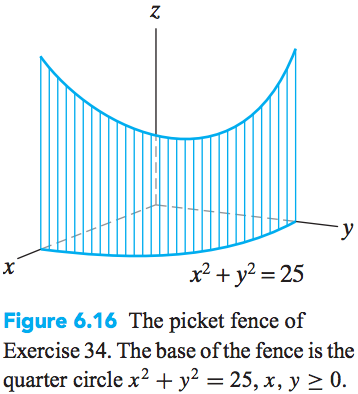
\includegraphics{img/6_1_34}
    \end{center}
\end{problem}
\begin{solution}
    \vfill
\end{solution}
\newpage

\begin{problem}[Colley 6.1.40]
    You are traveling through Cleveland, famous for its lake-effect
    snow in winter that makes driving quite treacherous. Suppose that
    you are currently located \SI{20}{miles} due east of Cleveland and
    are attempting to drive to a point \SI{20}{miles} due west of
    Cleveland. Further suppose that if you are $s$ miles from the
    center of Cleveland, where the weather is the worst, you can drive
    at a rate of at most $v(s)=2s+20$ miles per hour.
    \begin{enumerate}
        \item How long will the trip take if you drive on a
            straight-line path directly through Cleveland? (Assume that
            you always drive at the maximum speed possible.)
        \item How long will the trip take if you avoid the middle of
            the city by driving along a semicircular path with Cleveland
            at the center? (Again, assume that you drive at the maximum
            speed possible.)
        \item Repeat parts (a) and (b), this time using
            $v(s)=(s^2/16)+25$ miles per hour as the maximum speed that
            you can drive.
    \end{enumerate}
\end{problem}
\begin{solution}
    \vfill
\end{solution}
\end{document}
